%*************************************************************************************************************
% PREAMBLE STUFF
%*************************************************************************************************************
% Instead of inserting my \usepackage and defined commands here, I keep them in a separate file
% Queen's Thesis Format
% (Borrowed from Dean Jin's BigDis.tex file, then heavily modified :)

% Michelle L. Crane, Queen's University, 2003

%*************************************************************************************************************
% DOCUMENT STYLE
%*************************************************************************************************************
\documentclass[12pt]{report}
%-------------------------------------------------------------------------------------------------------------
\usepackage{quthesis}        % the Queen's University dissertation style file
                             % Note:  In my thesis, I had many Listings, so I
                             % tweaked the old quthesis sty file to create a
                             % List of Listings in the table of contents.
                             % However, this version of quthesis does *not*
                             % include these modifications.

%I don't even use the fancyheadings - it looks nice enough without it
%\usepackage{fancyheadings}  % doesn't seem to change the headings at all!
%*************************************************************************************************************


%*************************************************************************************************************
% SPACING
%*************************************************************************************************************
\usepackage{setspace}        % for use of \singlespacing and \doublespacing
%*************************************************************************************************************


%*************************************************************************************************************
% HEADINGS
%*************************************************************************************************************

% This changes the headings go that they are prettier, this can be commented out for traditional headings.
\usepackage{sectsty}
\allsectionsfont{\bfseries}% set all the section font to bfseries
\chapterfont{\centering\Large} % set the sizes of chapters, sections ...
\sectionfont{\normalsize}
\subsectionfont{\normalsize}

\usepackage{titlesec}
\titleformat{\chapter}[display]
  {\normalfont\bfseries}{}{0pt}{\Large}


% for formatting Table of Contents entry, example: Part 1 Introduction
\usepackage[subfigure]{tocloft}
\usepackage{tocloft}
\renewcommand{\cftchappresnum}{Part }
\renewcommand{\cftchapaftersnum}{:}
\renewcommand{\cftchapnumwidth}{7em}

%*************************************************************************************************************
% FOOTNOTES
%*************************************************************************************************************

\interfootnotelinepenalty=10000 % This line stops footnotes from splitting onto two pages.

%*************************************************************************************************************
% VERBATIM
%*************************************************************************************************************
\usepackage{moreverb}        % Using this package to get better control of the
                             % verbatim environment, mostly for the use of the
                             % listing environment which puts line number
                             % beside each line.  Note that there has to be a number
                             % in each set of brackets, i.e., \begin{listing}[1]{1}.
                             % PDF info file is "The moreverb package" by
                             % Robin Fairbairns (rf@cl.cam.ac.uk) after
                             % Angus Duggan, Rainer Schopf and Victor Eijkhout, 2000/06/29.
%-------------------------------------------------------------------------------------------------------------
%\usepackage{verbatim}        % allows the use of \begin{comment} and \end{comment}
                             % as well as \verbatiminput{file}
                             % Note:  when using verbatim to input from a text file,
                             % such as a specification or code, use \begin{singlespacing}
                             % and \end{singlespacing}.  Also, tabs are not read
                             % properly, so the input file must only use spaces.

%                             \begin{comment}
%                             Can also use the verbatim package for
%                             comments like this...
%                             \end{comment}
%*************************************************************************************************************

%*************************************************************************************************************
% INDEX
% Also possible to make an index; didn't use for my thesis.
%*************************************************************************************************************
%\usepackage{makeidx}         % to make the index
%-------------------------------------------------------------------------------------------------------------
% Tell Latex to make an index
%\makeindex
%*************************************************************************************************************


%*************************************************************************************************************
% MATH STUFF
%*************************************************************************************************************
\usepackage{amsmath}         % to make nice equations
%-------------------------------------------------------------------------------------------------------------
\usepackage{amsthm}          % to make nice theorem, i.e., definition

% Using the amsthm package, define a new theorem environment for my
% definition.  * means don't number it.
\newtheorem*{definition}{Definition}
%-------------------------------------------------------------------------------------------------------------
\usepackage{cases}           % to make numbered cases (equations)
%-------------------------------------------------------------------------------------------------------------
\usepackage{calc}            % Used with the Ventry environment defined below.
%*************************************************************************************************************


%*************************************************************************************************************
% FLOATS AND FIGURES
%*************************************************************************************************************
\usepackage{graphicx}        % for graphic images (use \includegraphics[...]{file.eps})
%-------------------------------------------------------------------------------------------------------------
\usepackage{subfigure}       % for subfigures (figures within figures)
%-------------------------------------------------------------------------------------------------------------
\usepackage{boxedminipage}   % to make boxed minipages, i.e., boxes around figures
%-------------------------------------------------------------------------------------------------------------
\usepackage{rotate}          % for use of \begin{sideways} and \end{sideways}
%-------------------------------------------------------------------------------------------------------------
\usepackage{float}           % Using this package to get better control of my floats
                             % including the ability to define new float types for
                             % my specification and code listings.
                             % DVI info file is "An Improved Environment for Floats"
                             % by Anselm Lingnau, lingnau@tm.informatik.uni=frankfurt.de
                             % 1995/03/29.

% Define new float styles here
% Ruled style for examples
%\floatstyle{ruled}
%\newfloat{Example}{h}{lop}[chapter]

% Style of float used for code listings
\floatstyle{ruled}
\newfloat{Listing}{H}{lis}[chapter]

                             % Note:  The listings don't have space between the chapters, unlike
                             % the standard list of tables etc.  At the end, copy the spacing
                             % commands from the .toc file and insert into the .lis file.  Then,
                             % DO NOT LATEX it again, simply go to the DVI
                             % viewer!
                             

%*************************************************************************************************************
% ALGORITHMS
%*************************************************************************************************************
\usepackage[ruled,vlined]{algorithm2e}
%*************************************************************************************************************
% TABLES
%*************************************************************************************************************
\usepackage{tabularx}        % Package used to make variable width-columns, i.e.,
                             % column widths are changed to fit the maximum width
                             % and text is wrapped nicely.

\usepackage{threeparttable}
\usepackage[graphicx]{realboxes}
%*************************************************************************************************************
% CAPTIONS
%*************************************************************************************************************
\usepackage[hang]{caption}   % Package used to make my captions 'hang', i.e., wrap
                             % around, but not under the name of the caption.
%-------------------------------------------------------------------------------------------------------------
% Find that the captions are too far from my verbatim figures, but if
% I change it to 0, then the captions are too close for my other types
% of figures.  Maybe set each one separately?
%\setlength{\abovecaptionskip}{1ex}

%\setlength{\textfloatsep}{1ex plus1pt minus1pt}

%\setlength{\intextsep}{1ex plus1pt minus1pt}

%\setlength{\floatsep}{1ex plus1pt minus1pt}
%*************************************************************************************************************


%*************************************************************************************************************
% MISCELLANEOUS
%*************************************************************************************************************
\usepackage{layout}          % useful for determining the margins of a document
                             % use with \layout command
%-------------------------------------------------------------------------------------------------------------
\usepackage{changebar}       % Way of indicating modifications by putting bars in the
                             % margin.  Read about it in "The Latex Companion".
%*************************************************************************************************************


%*************************************************************************************************************
% REFERENCES ETC.
%*************************************************************************************************************
\usepackage{varioref}        % Better page references, e.g., "on preceding page", etc.
                             % \vref{key} Create an enhanced reference.
                             % \vpageref[text]{key} Create an enhanced page reference.
                             % \vrefrange{key}{key} Create an enhanced range of references.
                             % \vpagerefrange[text]{key}{key} Create an enhanced range of page references.
                             % Note: doesn't really work for consecutive pages.

% Renewing the text for before and after, because I don't like the default flip-flopping one.
% And 'on the page before' sounds dumb!

\renewcommand{\reftextafter}{on the next page}
\renewcommand{\reftextbefore}{on the previous page}
%-------------------------------------------------------------------------------------------------------------
\usepackage{url}             % for use of \url - pretty web addresses
%*************************************************************************************************************
% HYPERLINKS (must be last)
%*************************************************************************************************************
%\usepackage[]{hyperref}
%\usepackage[dvips,bookmarks]{hyperref}
                             % Neat package to turn href, ref, cite, gloss entries
                             % into hyperlinks in the dvi file.
                             % Make sure this is the last package loaded.
                             % Use with dvips option to get hyperlinks to work in ps and pdf
                             % files.  Unfortunately, then they don't work in the dvi file!
                             % Use without the dvips option to get the links to work in the dvi file.

                             % Note:  \floatstyle{ruled} don't work properly; so change to plain.
                             % Not as pretty, but functional...
                             % The bookmarks option sets up proper bookmarks in the pdf file :)

% Need this command to allow hyperref to play nicely with gloss; otherwise
% almost every \gloss will cause an error...
%\renewcommand{\glosslinkborder}{0 0 0}
%*************************************************************************************************************


%*************************************************************************************************************
% MISCELLANEOUS COMMANDS AND ENVIRONMENTS
%*************************************************************************************************************
% Use this command to show more table of contents - used when playing
% with the draft outline
% I think it should be about 2???
\setcounter{tocdepth}{2}
%*************************************************************************************************************
% Environment definition I found in the "The Latex Companion".  Used to
% create a list environment where the indenting is the same for all of the
% entries, regardless of their length.  Note:  must \usepackage{calc}.
\newenvironment{Ventry}[1]%
    {\begin{list}{}{\renewcommand{\makelabel}[1]{\textbf{##1}\hfil}%
        \settowidth{\labelwidth}{\textbf{#1:}}%
        \setlength{\leftmargin}{\labelwidth+\labelsep}}}%
    {\end{list}}
%*************************************************************************************************************

%*************************************************************************************************************
% MY DEFINED COMMANDS
%*************************************************************************************************************
% Command that I can use to create notes in the margins;
% adapted from Juergen's META tag
%\newcommand{\meta}[1]{\begin{singlespacing}
%{\marginpar{\emph{\footnotesize Note: #1}}}\end{singlespacing}}
%*************************************************************************************************************
% Command that I can use to create lined headings
%\newcommand{\heading}[1]{\bigskip \hrule \smallskip \noindent \texttt{#1} \smallskip \hrule}
%*************************************************************************************************************
% Command that I can use for reading in a file, verbatim, with line
% numbers printed along the left side.  The parameter is the file name.
%\newcommand{\fileinnum}[1]{
%    \begin{singlespacing} {\footnotesize
%    \begin{listinginput}[1]{1}{#1}\end{listinginput}
%    }\end{singlespacing}
%}
%*************************************************************************************************************
% Command that I can use for reading in a file, verbatim, with NO line
% numbers, but in a smaller font.  The parameter is the file name.
\newcommand{\filein}[1]{
   \begin{singlespacing}{\footnotesize
    \begin{verbatiminput}{#1}\end{verbatiminput}
    }\end{singlespacing}
}

\newcommand{\specialcell}[2][c]{%
  \begin{tabular}[#1]{@{}l@{}}#2\end{tabular}}
%*************************************************************************************************************
% Command that I can use for reading in a file, verbatim, with NO line
% numbers, but in a smaller font.  The parameter is the file name.
\newcommand{\fileinsmall}[1]{
    \begin{singlespacing}{\scriptsize
    \begin{verbatiminput}{#1}\end{verbatiminput}
    }\end{singlespacing}
}
%*************************************************************************************************************
% Dean't 'notesbox' command.  Needs setspace package.
%   Usage: \notesbox{This is a note.}
%%
\newcommand{\notesbox}[1]{
     \ \\
      \singlespacing
      \noindent\begin{boxedminipage}[h]{\textwidth}{\sf{#1}}\end{boxedminipage}
      \doublespacing
}

\newcommand{\vect}[1]{\boldsymbol{#1}}


%*************************************************************************************************************
% INCLUDE ONLY
%*************************************************************************************************************
% Use if you want to include only certain parts of the document, example \includeonly{introduction}
% in order to speed up compile time when you're focussing on some particular part.
%\includeonly{}

%*************************************************************************************************************
% DOCUMENT
%*************************************************************************************************************

\begin{document}

%*************************************************************************************************************
% TITLE
%*************************************************************************************************************

\title{Stochastic Block Models for Modelling \\[1ex]Political Engagement}

\author{Cameron Raymond}

\dept{School of Computing}
\course{CISC 500 - Undergraduate Thesis}
\supervisor{Dr. Robin Dawes}

% OPTIONAL HERE
% ~~~~~~~~~~~~~
% \submitdate{month year in which submitted to GPO}
%        - date LaTeX'd if omitted
% \copyrightyear{ear degree conferred}
%        - year LaTeX'd if omitted
% \figurespagetrue or \figurespagefalse
%        - produce or don't produce a List of Figures page (true by default)
\figurespagefalse
% \tablespagetrue or \tablespagefalse
%        - produce or don't produce a List of Tables page (true by default)
\tablespagefalse

\beforepreface

% Adding single spacing so abstract and table of contents is single spaced.

%*************************************************************************************************************
% ABSTRACT
%*************************************************************************************************************

\prefacesection{Abstract}

The advent of social media has enabled political parties to engage with the
broader populous in new and unforeseen ways. This, coupled with rising levels of
political polarization has prompted debates as to whether people care about
policy anymore, or if they self-select into political bubbles online based on
their chosen party leader. This thesis proposes a novel adaptation of stochastic
blockmodelling to measure the degree to which political engagement on Twitter is
driven by policy or party leaders. Building on a graph theoretical approach,
measures of topic centrality are developed to give a metric for how efficient
topics were at either rallying or spanning party leaders' bases. This is done in
the context of the 2019 Canadian federal election.


%*************************************************************************************************************
% CO-AUTHORSHIP (if necessary)
%*************************************************************************************************************

%\prefacesection{Co-Authorship}

%*************************************************************************************************************
% ACKNOWLEDGEMENTS
%*************************************************************************************************************

\prefacesection{Acknowledgments}

Blah blah blah.


\singlespacing \afterpreface \doublespacing

% Include my chapter texts - kept separated to make editing easier.
\chapter{Introduction}

\section{Background}

The advent of social media has enabled political parties to engage with the
broader populous in new and unforeseen ways. The ability to bypass the
traditional mediating forces of mass media allows for an unfiltered promotion of
policy, ideology and party stances. This is specifically interesting in Canada’s
political system which has historically been defined by large brokerage parties.
In order to win a diverse range of electoral districts across Canada, these “big
tent” parties try to appeal to various political persuasions. Political adverts,
and policy have traditionally been the conduits through which brokerage parties
attempt to accommodate different ideologies, but social media allows for a
direct, granular approach to political messaging which is completely novel.
Social networks, formed through new media like Twitter, are inherently
relational and thus lend themselves well to being represented as graphs.
Therefore, as political strategy becomes increasingly digital, the use of graph
theory can potentially illustrate how large brokerage parties organize and along
what axes Canadians engage with political parties.

\section{Motivation}\label{sec:motivation}

The way information is distributed and received has changed significantly over
the past decade. Cogburn and Espinoza-Vasquez argue that Barrack Obama’s 2008
presidential campaign was a watershed moment in social media campaigning -- and
in the subsequent decade, from Macron to Brexit to the Five Star Movement,
social media has played an increasing role in how politics is conducted
\cite{cogburn2011networked}. Between 2013 and 2018, the share of Canadian
federal media expenditure spent on digital advertising rose from 27\% to 65\%, a
140\% increase, making the study of new media critical from a social science
perspective \cite{annualReportCanadaAdvertisingActivities_2018}. Additionally,
rises in political polarization, populism and a decline in trust in political
institutions in the $21^{st}$ century has been a topic of popular debate. Ezra
Klein argues in his 2019 book, \emph{Why We're Polarized}, that this due to a
shift in preferences for parties over policies \cite{levitsky2018democracies}.
If this is the case, then this preference to engage along party lines rather
than choosing to engage with specific issues should pattern engagement. An
empirical analysis of how users behave and engage with political parties online
should privilege the relational aspect of social media. Social network analysis
helps avoid the pitfalls of survey data, famously described by Allen Barton as
``a sociological meat grinder, tearing the individual from [their] social
context'' \cite{freeman2004development}.

Graph theory’s use in social network analysis, also called network science, has
already been applied to explore problems in marketing, sociology and
epidemiology -- but there is a gap in analysis of political engagement online.
Therefore, the contribution of this thesis is a novel, robust mathematical
process for analyzing different axes of political engagement online in a purely
relational manner. A secondary outcome of making relationships a “first-class
citizen” in this work will be an organic analysis of what issues produce the
most engagement. This deviates from traditional survey data that ask test
subjects which issues concern them -- and instead uses observations of past
behaviour to model variations in local connectivity to answer the question:“what
do people actually care about?”All of this will be done in the context of the
2019 Canadian federal election and the tweets of Canada's five major, english
speaking party leaders: Andrew Scheer, Elizabeth May, Jagmeet Singh, Justin
Trudeau, and Maxime Bernier. 

\section{Research Question}

The primary question concerning this project is: in the lead up to the 2019
Canadian federal election, did politically active users on Twitter engage with
political elites along the axis of issues\footnote{The terms policy, issue and topic will be used interchangeably to
refer to categories of messages.} or parties? If Ezra Klein is correct, then \emph{who} produces the
message will pattern engagement more than \emph{what} the message is; this will
act as the initial null hypothesis, with the alternate hypothesis being that who
produces the message is equally to or less important than what the message is. 

The secondary question to be explored is: during this period, what topics
produced the highest level of engagement? Also, what topics spanned
multiple party leaders' bases, indicating a bridging of different ideologies,
and what topics rallied party leaders' bases?
\chapter{Social Media and Politics}\label{ch:SMandPolitics}

\section{Political Communication in the Digital Era}

Technological innovation often precedes political disruption; Martin Luther’s 95
theses could only be spread at scale by virtue of Gutenberg inventing his
printing press first \cite{gardels2019renovating}. This example had obvious
political ramifications and is a testament to the impact of the means of
communication on the political sphere. McNair defines political communication
as:

\begin{enumerate}    
    \item All forms of communication undertaken by politicians and other
    political actors for the purpose of achieving specific objectives.
    \item Communication addressed to these actors by non-politicians such as
    voters and newspaper columnists.
    \item Communication about these actors and their activities, as contained in news reports, editorials, and other forms of media discussion of politics. \cite{mcnair2017introduction}
\end{enumerate} 

This is a broad, outward focused definition that includes most public, political
discourse -- verbal or otherwise. However, social media has changed all three
aspects of this definition in novel ways. Most notably, the rate at which
politicians can communicate information to achieve “specific objectives” has
increased as a result of rapid nature of social media, and the granularity at
which actors can target the these messages has gotten smaller due to the massive
swaths of user data available \cite{nickerson2014political}. Therefore, the
value of using computational methods to study political communication in the
$21^{st}$ century is a natural fit.

\subsection{Technology's Implications for Democratization}

While fully exploring the impact of social media on democracy is out of the
scope of this project, it is an important justification for why research in this
area needs to be conducted. The traditional model of the media being a mediating
force through their reporting, commentary and analysis is no longer valid.
Previously, political actors needed to use the media to broadcast their messages
to their desired audiences \cite{mcnair2017introduction}. Social networking
sites allow these same actors to reach audiences in the millions without having
to gain access to the media first; in this effect, the second and third elements
of McNair’s definition are also being transformed. Yascha Mounk argues that this
has given voice to political outsiders who would be shut out from mainstream
platforms. Thus, social media may not be inherently democratic or undemocratic,
as it has contributed to democratic backsliding and overturning authoritarian
governments, but it can certainly have a destabilizing affect
\cite{mounk2018people}. Therefore, a better understanding of new media’s
ramifications is critical, and empirical modeling can aide in this
understanding.

\section{Canadian Brokerage Politics}

While it is clear that technology is changing how information is received, and
thus must also be changing how politics is conducted, it may not be clear the
role of Canadian politics in this research. However, Canada’s political system
is the perfect environment to test the importance of political messaging,
because relative to most liberal democracies, the system is dominated by party
politicians. As Carty put it:

\begin{quote}
No obvious simple geographic reality, no common linguistic or religious
homogeneity, no common revolutionary experience or unique historical moment
animated [Canada] or gave it life. Canada was created when a coalition of party
politicians deemed it to be in their interest to do so, and it has been
continuously grown, reshaped and defended by its politicians.
\cite{carty2010political}
\end{quote}

Thus, it is not surprising that Canada’s electoral system encourages electoral
pragmatism -- and developed large, “big tent” parties that are among the most
organizationally weak and decentralized of established democracies
\cite{carty2010political}. This system defines political parties as brokers of the
often conflicting, weakly integrated electorate -- as opposed to mobilizers of
distinct communities, articulating claims rooted in their pre-existing
interests. In this way, parties act as the principal instruments of national
accommodation, rather than democratic division \cite{carty2010political}.

\subsubsection{Rationale}

The dominance of parties in Canadian politics, their amorphous ideological
stances, and the many intersectional geographic, linguistic and religious
cleavages have given birth to what’s been coined the brokerage party system.
\cite{carty2010political}. The need to capture pluralities in a diverse range of
electoral districts gives Canada a unique set of dynamics - making it an
interesting case to explore.

\chapter{Modelling Unstructured Text Data}\label{ch:TopicModelling}

\section{Background}

The majority of data currently being produced is unstructured and unclassified,
and much of it is in the form of text. As a result, there is a need for
techniques that autonomously organize big, unclassified corpuses of text. Topic
modeling finds clusters of words that frequently occur together (topics),
connects words with similar meanings, and distinguishes different uses of words
with multiple meanings \cite{alghamdi2015survey}. This is based on the
underlying assumption that a document is concerned with a fixed set of topics,
and that the frequency of words used is indicative of this latent structure
\cite{blei2003latent}. Topic modeling has been used extensively to create
recommendation systems, perform trending analysis, and segment text
\cite{alghamdi2015survey}. In this context, topic modeling is necessary to
organize the tweets party leaders are promoting by their latent topics. The
ultimate goal of evaluating along what axes the broader populous engages with
political media (policies/topics/issues or party lines) necessitates a robust
way of evaluating messages. To know how people engage politically based on
various topics requires knowing what those topics are in the first place. Topic
extraction approaches based on keywords are brittle, context specific and are
unable to capture emergent topics. Using unsupervised machine learning
techniques, like the latent Dirichlet allocation discussed in section
\ref{sec:LDA}, topics are able to be extracted in an autonomous manner -
requiring little oversight.

\section{Latent Dirichlet Allocation}\label{sec:LDA}

Blei, Ng and Jordan describe latent Dirichlet allocation (LDA) as a “generative
probabilistic model for collections of discrete data such as text corpora.” The
goal being to extract short descriptions of similar topics from a collection -
and describe statistical relationships that are useful for classification,
summarization, and describing similarity \cite{blei2003latent}. The underlying
thought process behind the LDA is that each document in a corpus can be
described as a distribution of topics, and that each topic can be described as a
distribution of words. 

In this process, each unique word in the text corpus is an element of the
vocabulary, $Voc: \{1,...,V\}$. Each word, $v\in V$, is represented by $w$, a
unit-basis vector of dimension $V$ where:

\begin{numcases}{\text{$w[index=i]$}}
    1   & if $v = i$ \notag \\
    0   & if $v \neq i$ \notag
\end{numcases}

A document is a sequence of $N$ words denoted by $\vect{w} =
(w_{1},w_{2},...,w_{N})$. A corpus is a collection of $M$ documents denoted by
$D = \{\vect{w_{1}},\vect{w_{2}},...,\vect{w_{M}}\}$. 

The input to LDA, $D$, will be the tweets aggregated and cleaned from the
federal Canadian party leaders described in section \ref{sec:motivation}. Aside
from the corpus and $k$ - the number of topics - two other parameters are fed to
the LDA. First, $\alpha$, which is organizes the ground $\theta$, a Dirichlet
distribution, and acts as a concentration parameter for how documents are
modelled as topics. Higher $\alpha$ values generally implies that documents will
be viewed as a mixture of topics, whereas low $\alpha$ values imply that
documents will be viewed as a belonging to a single topic. Similarly, to model
words as topics the parameter $\eta$ organizes the ground for $\beta$, a
Dirichlet distribution. 

The generative model for the LDA uses $\theta$ to choose a topic $z_{n}$ of the
$k$ topics that the next word will reside from, and then chooses a word $w_{n}$
from $p(w_{n} |z_{n},\beta$), a multinomial probability conditioned on the topic
$z_{n}$. This processes is described graphically in figure \ref{fig:lda_fiugre}

\begin{singlespacing}
    \begin{figure}[H]
    \centering
    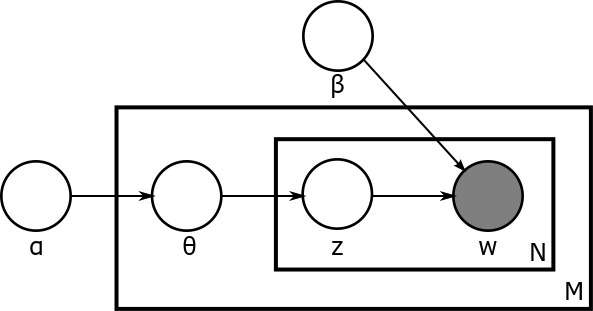
\includegraphics[scale=0.4]{Figures/lda_figure}
    \caption[Graphical Model of the Latent Dirichlet Allocation]{Graphical Model of the Latent Dirichlet Allocation}
    \label{fig:lda_fiugre}
    \end{figure}
\end{singlespacing}

By using variational inference - $\theta$, a distribution of topics for each
document and $\beta$, a distribution of words (one for each topic) can be solved
for giving the final equation
$P(\theta_{1:M},\vect{z}_{1:M},\beta_{1:k}|D,\alpha_{1:M},\eta_{1:k})$
\cite{blei2003latent}.
\chapter{Graph Theory and Computational Social Science}\label{ch:GraphTheory}

Graph theory is the study of mathematical structures, called graphs, which are
used to model pairwise relations between entities. Graphs consist of a finite
set of vertices, $V$, and a set of ordered pairs of vertices, $E$, called edges.
A graph can be defined by the tuple, $G=(V,E)$. The graphs built in this project
have added constraints and is defined as below:

\begin{itemize}
    \item \emph{Vertices}: Let $V_{1}=\{v_{1},v_{2},...,v_{n}\}$ be the set of
    party leaders; $V_{2}=\{v_{1},v_{2},...,v_{m}\}$ be the set of tweets by the
    party leaders described in section \ref{sec:motivation}; and let
    $V_{3}=\{v_{1},v_{2},...,v_{k}\}$ be the set of users who retweet tweets.
    Let the total set of vertices, $V$, be equivalent to $V_{1}\cup V_{2}\cup
    V_{3}$.    
    \item \emph{Edges}: Let $E$ be the set of edges. Allow the edge $(v_{1},
    v_{2})\in E$ if and only if $v_{1}\in V_{1}, v_{2}\in V_{2}$ or $v_{1}\in
    V_{3}, v_{2}\in V_{2}$. By this definition, we will only allow edges from a
    party leader vertex to a tweet vertex, or from a“retweeter” vertex to a
    tweet vertex.
\end{itemize}

\section{Spectral Graph Theory}\label{sec:spectralGraphTheory}

Spectral graph theory studies the structures of graphs via the eigenvectors of
their adjacency matrix, Laplacian matrix, or some other variant of the two. The
set of eigenvalues for a graph if size $n$, $\{\lambda_{1},...,\lambda_{n}\}$,
is called the spectrum of a graph \cite{netlsd}. As Hammond et al. note, graph
spectra are closely related to major graph invariants \cite{chung1997spectral}.
Graph spectra have been used in image segmentation and object recognition tasks,
as well as in studying the stability of molecules; Elghawalby and Hancock
demonstrated how the euclidian distance between graphs' spectra track the edit
distances between graphs \cite{elghawalby2008measuring,chung1997spectral}. As
such, spectral graph theory is useful in comparing the underlying structure of
two graphs -- allowing for nuanced distance and similarity metrics.   

\subsection{Network Laplacian Spectral Descriptor}\label{sec:NetLSD}

While various distance metrics are tracked by graph spectra, most are not size
invariant or scale adaptive. Size invariant similarity metrics capture that two
graphs that are structurally similar as close together, regardless of magnitude.
Scale adaptive similarity metrics would be able to capture both local and global
features of a graph. Tsitsulin et al. developed the Network Laplacian Spectral
Descriptor (NetLSD), a state of the art similarity measure, that creates
extracts a compact heat trace signature from a graph's normalized Laplacian
spectrum using the heat kernel \cite{netlsd}. This, in effect, models how heat
diffuses throughout a network over; with local features being captured in the
immediate time-steps after the nodes are ``heated'' (and only affecting adjacent
nodes) and global features being captured as heat becomes further diffuse.
Figure~\ref{fig:heat_trace_ex} shows how the two graphs can be similar at a
global level and local level, but differ at an intermediate scale \cite{netlsd}.

\begin{singlespacing}
    \begin{figure}[H]
    \centering
    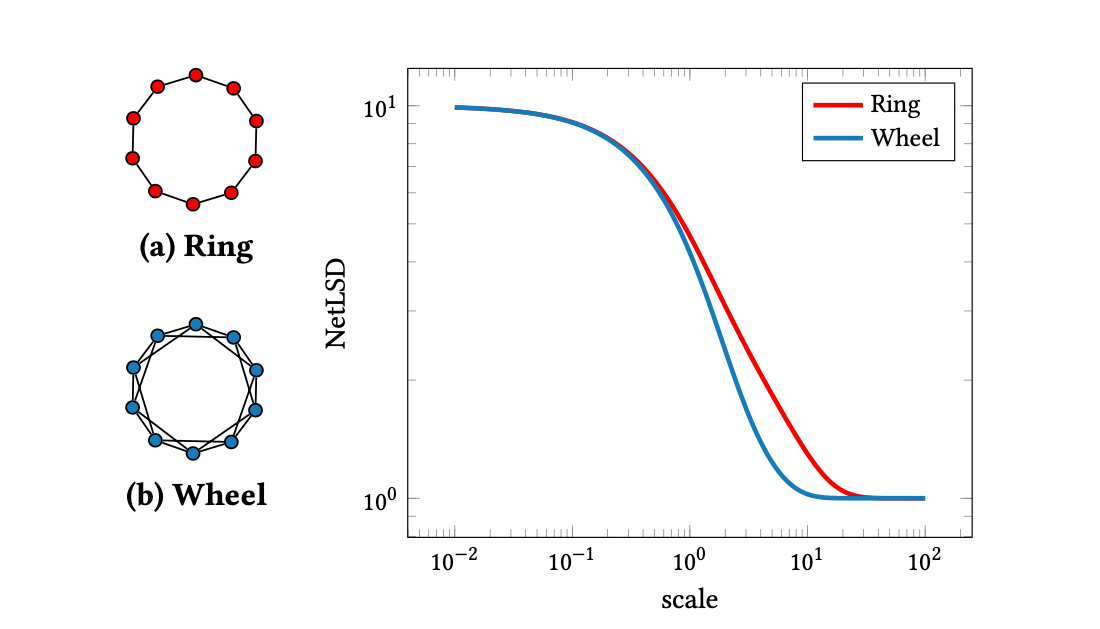
\includegraphics[scale=0.25]{Figures/heat_trace_ex}
    \caption[NetLSD Heat Trace Signatures for two Similar Graphs \cite{netlsd}]{NetLSD Heat Trace Signatures for two Similar Graphs \cite{netlsd}}
    \label{fig:heat_trace_ex}
    \end{figure}
\end{singlespacing}

The heat trace ($h_{t}$) for a graph at time $t$ is calculated by taking the
eigenvalues of the graph's normalized Laplacian matrix, and summating their
exponentiation multiplied by $-t$. 

\begin{equation}\label{equation:heat_trace}
    h_{t}=\sum_{j}^{n}e^{-t\lambda_{j}}
\end{equation}
 
Given that a graph with $n$ nodes will have $n$ eigenvalues and thus have a
higher heat trace value at any given time -- the heat trace can be normalized
against an empty graph, which has all zero eigenvalues \cite{netlsd}. The
\emph{heat trace signature} then is a vector of different heat traces at
different times denoted by $h(G)$:

\begin{equation}\label{equation:heat_trace_sig}
    h(G) = \{h_{t}\}_{t\geq0}
\end{equation}

Two graphs can be compared via the $L_{2}$ distance among trace signatures.

\section{Random Graphs}\label{sec:RandomGraphs}
    
Real world interactions are not deterministic. That is -- who your friends are,
whether you contract a disease, or whether you choose to retweet a tweet are the
result of random processes, patterned by your connections with others.
Therefore, modelling how social networks form requires investigating the
underlying of the processes that generate these random ties. As Robins'
discusses in his article,\emph{ a tutorial on methods for the modeling and
analysis of social network data}, graphs where edges are generated in some
stochastic process can help illustrate how relationships drive behaviour
\cite{robins2013tutorial}.  

\subsection{Stochastic Blockmodels}\label{sec:SBM}

Initially, random graph models were primarily developed to ``model  variations
in local connectivity of each network actor, the degree of local clustering
among actors, and the general distribution of connectivity."
\cite{robins2013tutorial} However, intrinsic characteristics of actors in a
network often patterns the relationships found; inter vs intra-group dynamics
drive Shakespeare's Romeo and Juliet, and how the characters behaved was largely
determined by which family they were a part of \cite{doreian2005generalized}.
Blocks therefore group all nodes of the same characteristics. The proportion of
all possibles edges within a group -- and the proportion of all possible edges
that span to all other blocks -- formulate the probabilities of forming edges in
the generative blockmodel. Figure \ref{fig:blockmodel_ex} visualizes a
friendship network with each node (representing a person) coloured according to
their sex, and edges between nodes denoting friendship between them.

\begin{singlespacing}
    \begin{figure}[H]
    \centering
    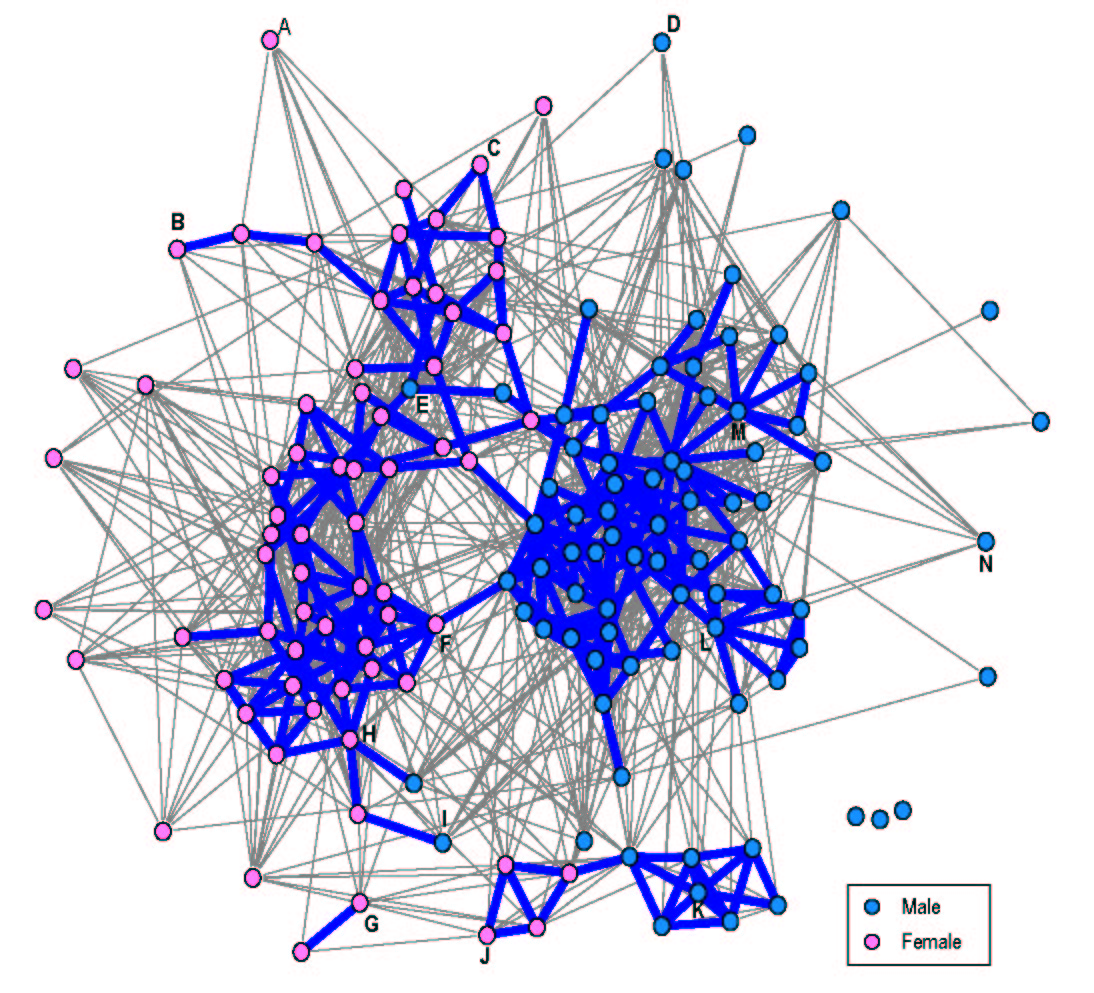
\includegraphics[scale=0.2]{Figures/blockmodel_ex}
    \caption[Friendship Blockmodel With Nodes Coloured by Sex]{Friendship Blockmodel With Nodes Coloured by Sex}
    \label{fig:blockmodel_ex}
    \end{figure}
\end{singlespacing}

Of all the possible edges for a network of that size, the ones observed are
overwhelmingly between members of the same sex, with fewer edges spanning that
characteristic. These are attributes that shape behaviour that blockmodels
attempt to capture. 

Stochastic blockmodelling, first proposed by Holland et al. in 1983, is a subset
of blockmodels that takes classes of nodes to be latent
\cite{holland1983stochastic}. The goal, therefore, of stochastic blockmodels are
to determine the latent classes necessary to define the blockmodel. 

For the purposes of this thesis, stochastic blockmodels will be adapted and
extended to capture how users on Twitter show preferences for party leaders
and/or policies when deciding whether to engage with tweets. The model will have
to realistically model the spectrum of users; from those who only engage with
one party leader, to those who retweet multiple party leaders, to those whose
engagement driven by specific issues. 
	
\section{Measures of Centrality}

Centrality is a measure of prominence for vertices within a graph. For the
purpose of this thesis, it will be used to measure the relative importance of
different topics tweeted about in the lead up to Canada's 2019 federal election.

\subsection{Background}\label{sec:CentralityBackground}

There are various different ways of measuring vertex centrality that have
successfully been applied to problems in marketing, economics and epidemiology;
Stephenson and Zelen explored the utility of centrality measures in studying the
social dynamics of Gelada baboons. \cite{stephenson1989rethinking}. Common
centrality measures include measures of degree and betweenness. This thesis will
focus on the notion that central vertices are close to other central vertices,
which is one of the founding intuitions behind Google’s “page-rank” algorithm
and eigenvector centrality. 

\subsection{Eigenvector Centrality}\label{sec:EigCentrality}

As Newman lays out in his 2016, Mathematics of Networks: ``the eigenvector
centrality [...] accords each vertex a centrality that depends both on the
number and the quality of its connections: having a large number of connections
still counts for something, but a vertex with a smaller number of high-quality
contacts may outrank one with a larger number of mediocre contacts.''
\cite{newman2008mathematics}

If we define the eigencentrality of vertex $x$ as $C_{E}(x)$, where $C_{E}(x)$
is proportional to the average eigenvector centrality of $x$'s neighbours,
multiplied by some constant $\lambda$:
\begin{equation}
    C_{E}(x)=\frac{1}{\lambda}\sum_{j=1}^{n}A_{xj}C_{E}(x)
\end{equation}
By defining the vector of centralities as $C_E(X) = (C_E(x_1),C_E(x_2),...)$
this equation can be rewritten as $\lambda C_E(X) = \lambda A$, and it is
evident that CE(V) is an eigenvector of the adjacency matrix with eigenvalue,
$\lambda$ \cite{newman2008mathematics}. By Perron-Frobenius theorem, picking the
largest eigenvalue of $A$ will result in all elements of $C_E(X)$ being
non-negative \cite{newman2008mathematics}.

\chapter{Thesis Contribution}\label{ch:ThesisCont}
      
\section{Topic Modelling}\label{sec:TopicModelling}

In order to evaluate the relative importance of policy and party leaders in
driving political engagement on Twitter, all the tweets collected must first be
organized by topic. In order to do so, a latent Dirichlet allocation (LDA) was
trained on the English tweets of Canada's five major, english speaking party
leaders: Andrew Scheer, Elizabeth May, Jagmeet Singh, Justin Trudeau, and Maxime
Bernier. The timeframe of collection ranges from October 21, 2018 to October 21,
2019 - the eve of Canada's federal election. While the tweets from each Federal
party's official Twitter accounts were also collected, they predominantly acted
as logistical tools -- informing party affiliates of events and rallies. The
personal accounts for party leaders were generally more pertinent to their
beliefs, platforms and style of rhetoric, and thus are better suited in this
context. In this spirit, only tweets of the party leader were used, excluding
retweets. Figure \ref{fig:tweets_over_time} visualizes the daily and cumulative
number of tweets over time, in aggregate and by party leader, resulting in 7978
total tweets.

\begin{singlespacing}
    \begin{figure}[H]
    \centering
    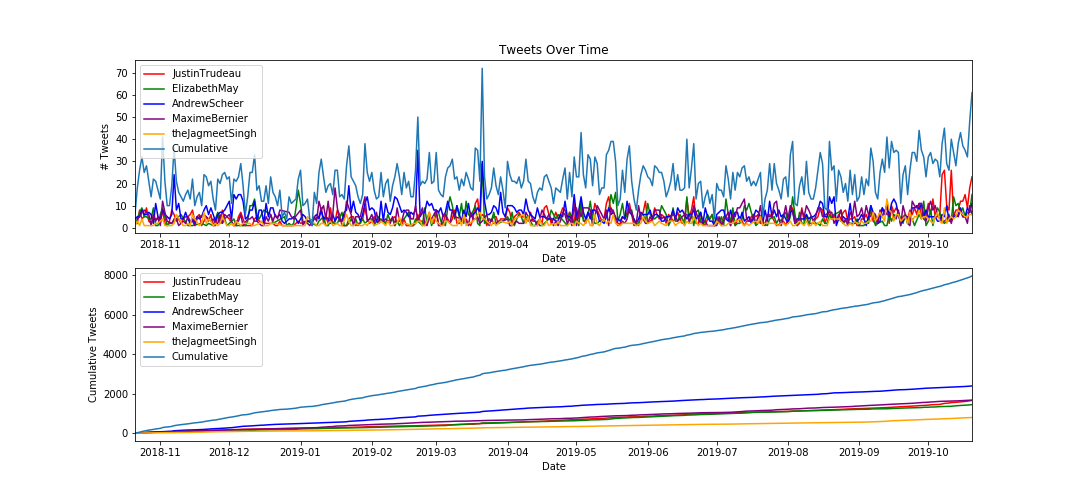
\includegraphics[scale=0.40]{Figures/tweets_over_time}
    \caption[Daily and Cumulative Tweets over Time]{Daily and Cumulative Tweets over Time}
    \label{fig:tweets_over_time}
    \end{figure}
\end{singlespacing}

\subsubsection{Text Cleaning}

Given the inherent noise and extraneous info in text data, it is standard and
necessary to preprocess text before modelling \cite{sapul2017trending}. The text
cleaning pipeline removes punctuation marks, stop words, words with fewer than
three characters, and URLS, as well as common twitter symbols like ``RT:'',
``@'' and ``\#''. Emojis were converted to text using the python package
\texttt{emoji}. After this process, all text was converted to lower-case and
lemmatized to get rid of common suffixes. Therefore the tweet in figure
\ref{fig:tweet_ex} after preprocessing reads: \emph{wherever maple leaf fly
represents rich history bright future value hold dear happy flag day canada}.

\begin{singlespacing}
    \begin{figure}[H]
    \centering
    
\includegraphics[scale=0.55]{Figures/tweet_ex}
    \caption[Example Tweet]{Example Tweet}
    \label{fig:tweet_ex}
    \end{figure}
\end{singlespacing}

\subsection{Hyper-Parameter Tuning}\label{sec:TopicModellingHP}

As discussed in section \ref{ch:TopicModelling}, the LDA takes in three
parameters: $\alpha$ - which acts as a concentration parameter for how documents
are modelled as topics; $\beta$ - which acts as a concentration parameter for
how topics are modelled as words; and $k$ which is the number of topics to be
modelled. By performing a parameter sweep, where $\alpha$ and $\beta$ lie on the
interval $\left[0,1\right]$ with increments of 0.05, and $k$ ranges between 4
and 7, the LDAs were exposed to the entire corpus and then evaluated using c\_v
coherence. Figure \ref{fig:lda_param_sweep} shows, for each $k$ value, the c\_v
coherence as a function of different combinations of $\alpha$ and $\beta$.

\begin{singlespacing}
\begin{figure}
    \centering
    \begin{tabular}{cc}
      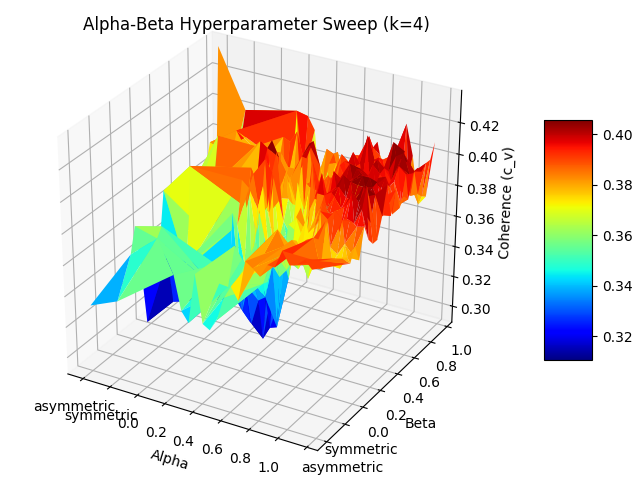
\includegraphics[width=65mm]{Figures/Coherence_Surface_k=4} &
      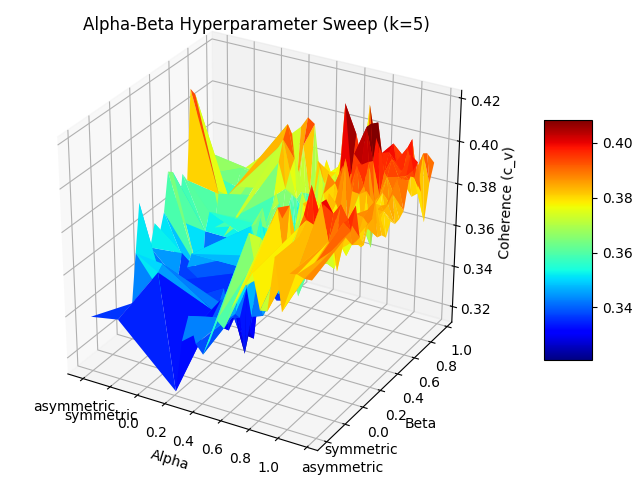
\includegraphics[width=65mm]{Figures/Coherence_Surface_k=5} \\
    (a) $k=4$ & (b) $k=5$ \\[6pt]
     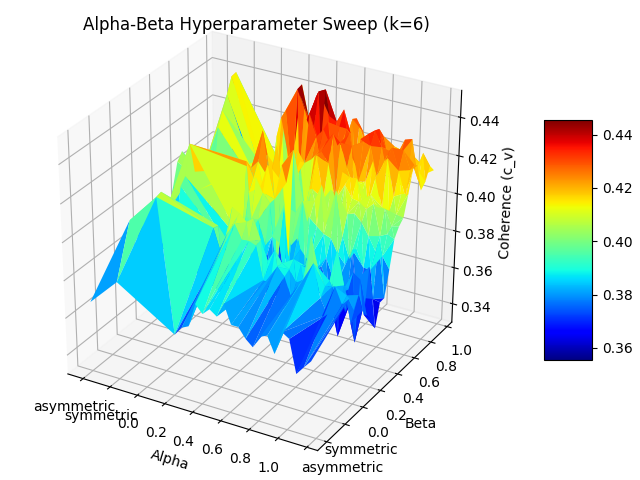
\includegraphics[width=65mm]{Figures/Coherence_Surface_k=6} &
     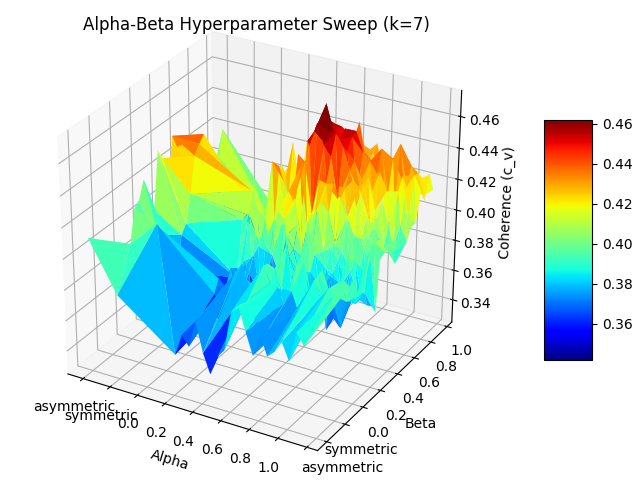
\includegraphics[width=65mm]{Figures/Coherence_Surface_k=7} \\
    (c) $k=6$ & (d) $k=7$ \\[6pt]
    \end{tabular}
    \caption[LDA Parameter Sweep Results]{LDA Parameter Sweep Results}
    \label{fig:lda_param_sweep}
\end{figure}
\end{singlespacing}


\subsection{Results}\label{sec:TopicModellingRes}

After performing the parameter sweep described in section
\ref{sec:TopicModellingHP}, the most performant model had a $k$ value of 7,
$\alpha$ of 0.31 and $\beta$ of 0.81 and a c\_v coherence score of 0.48. By
labelling each tweet as the maximum probability value in its topic mixture, each
tweet was assigned a single topic. The word clouds for each topic are described
in figure \ref{fig:topic_word_clouds}. 

\begin{singlespacing}
    \begin{figure}
        \centering
        \begin{tabular}{ccc}
        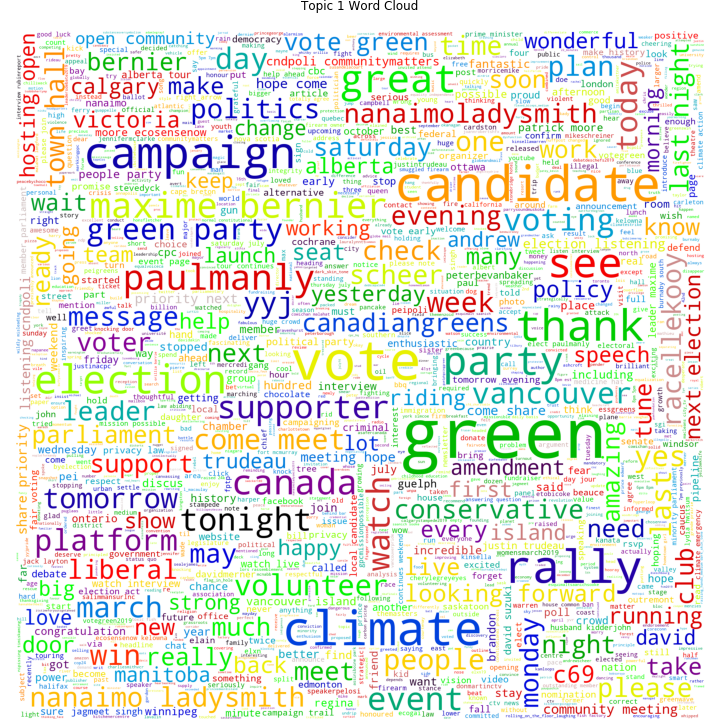
\includegraphics[width=45mm]{Figures/topic_1_wordcloud} &
        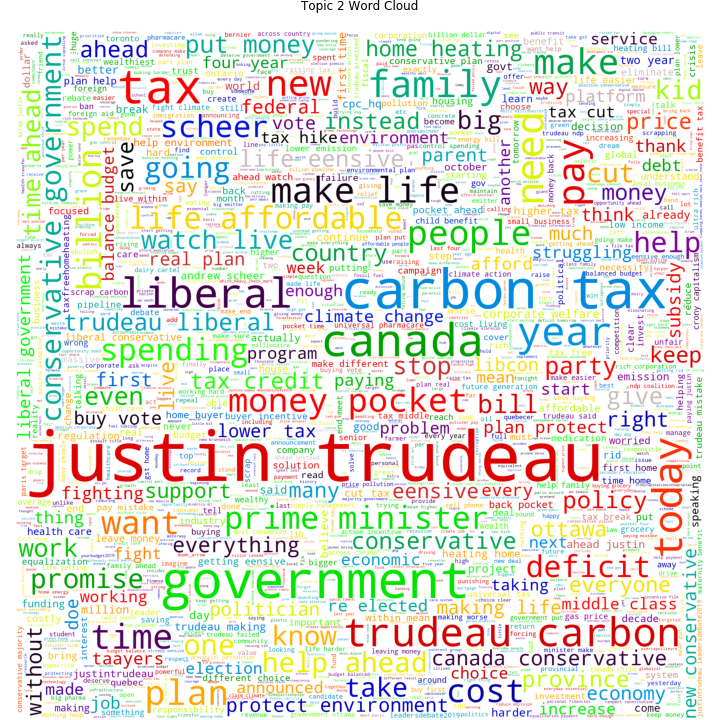
\includegraphics[width=45mm]{Figures/topic_2_wordcloud} &
        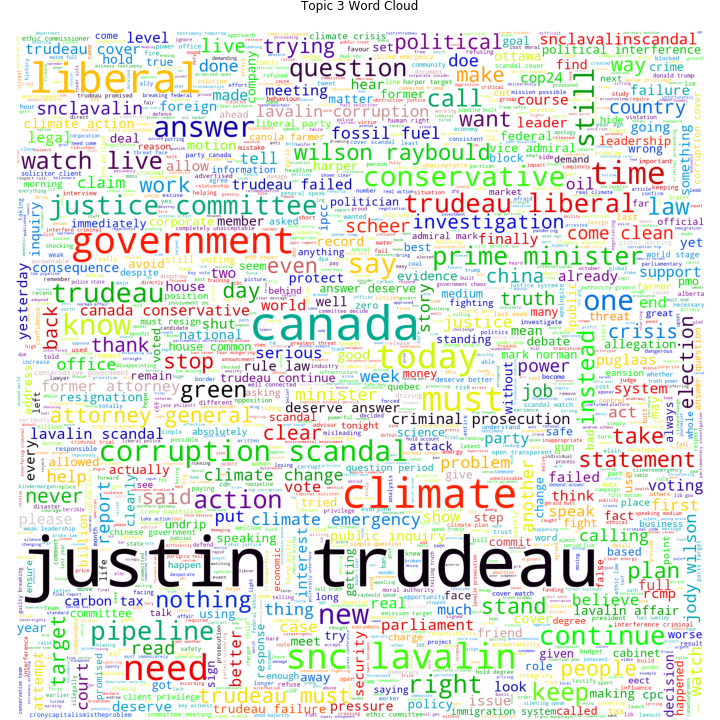
\includegraphics[width=45mm]{Figures/topic_3_wordcloud} \\
        (a) Topic 1 & (b) Topic 2 & (c) Topic 3  \\[6pt]
        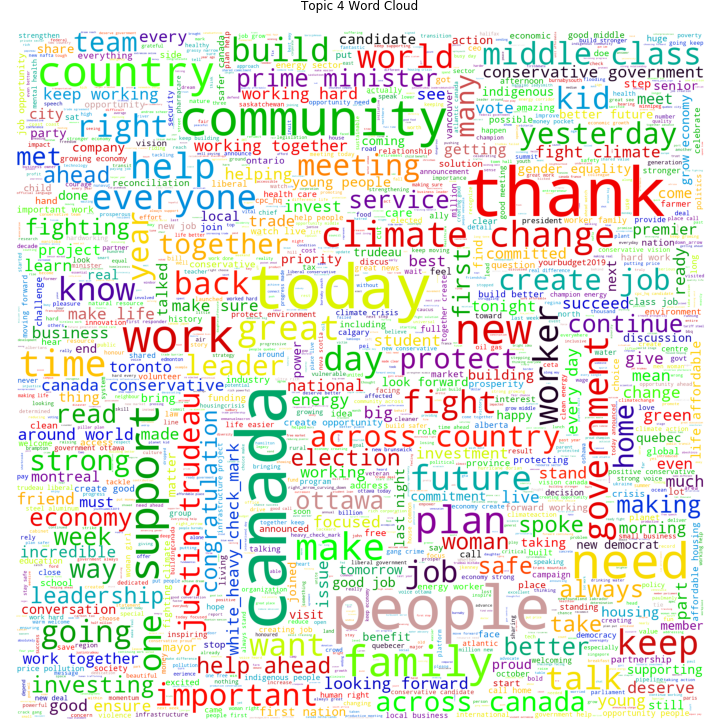
\includegraphics[width=45mm]{Figures/topic_4_wordcloud} &
        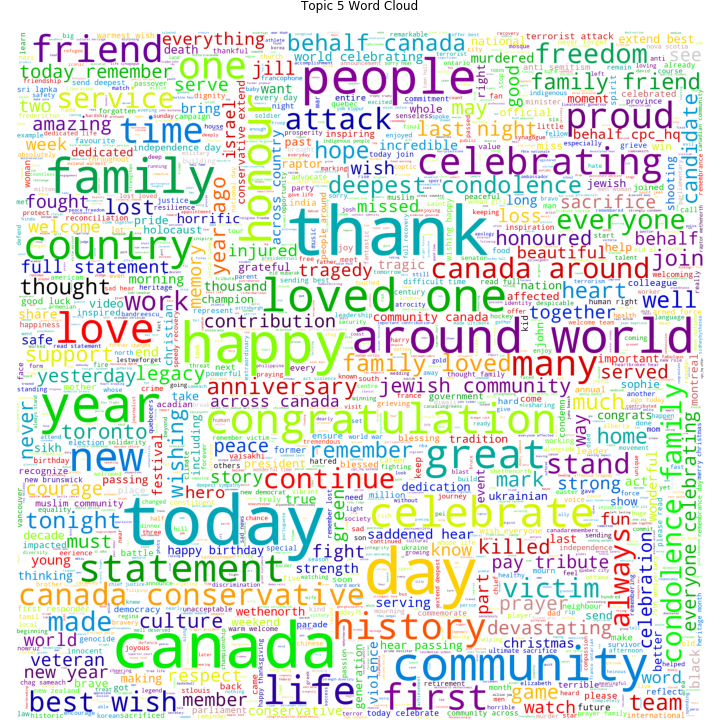
\includegraphics[width=45mm]{Figures/topic_5_wordcloud} &
        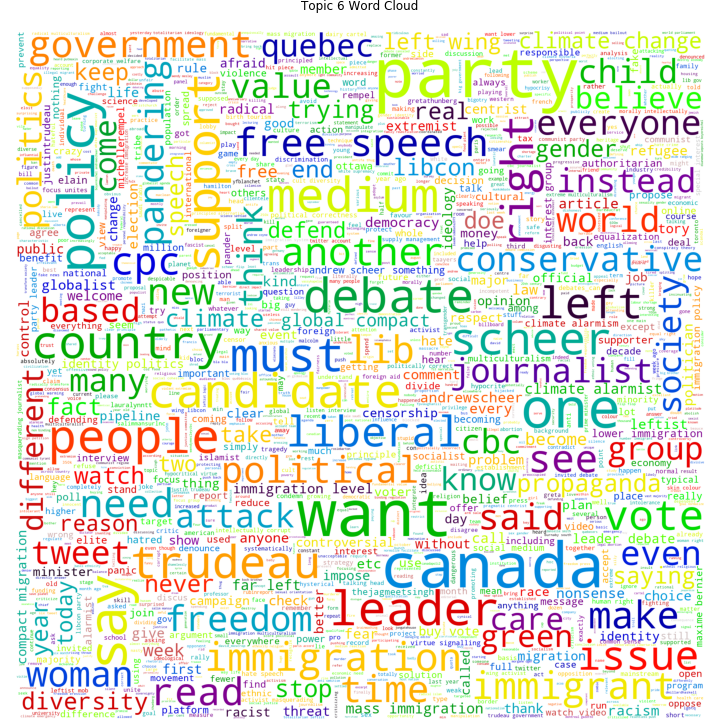
\includegraphics[width=45mm]{Figures/topic_6_wordcloud} \\
        (d) Topic 4 & (e) Topic 5 & (f) Topic 6  \\[6pt]
        \multicolumn{3}{c}{
\includegraphics[width=45mm]{Figures/topic_7_wordcloud}
        }\\
        \multicolumn{3}{c}{(g) Topic 7}
        \end{tabular}
        \caption[LDA Topic Word Clouds]{LDA Topic Word Clouds}
        \label{fig:topic_word_clouds}
    \end{figure}
\end{singlespacing}

Topic 1 pertained to campaign messages, rallies and logistics -- and makes up
8.2\% of all tweets. Topic 2 contains tweets regarding a carbon tax, pipelines
and the economy -- and makes up 16.3\% of all tweets. Topic 3 contains tweets
about the SNC Lavalin affair, a scandal that plagued Justin Trudeau, and tweets
about corruption -- making up 18\% of all tweets. Topic 4 is predominantly
tweets appealing to the middle-class and economy -- and is 29.7\% of all tweets;
topic 5 contains celebratory messages about the campaign, as well as tweets
regarding national holidays and days of remembrance -- and make up 15\% of all
tweets. Topic 6 is made up of tweest about immigration, diversity and free
speech -- and makes up 11.5\% of all tweets. Finally, topic 7 contains tweets
regarding healthcare, abortion and pharmacare -- and makes up 1\% of all tweets.
The magnitude of how many tweets were assigned to each topic is shown in figure
\ref{fig:topic_distribution}. The vertices representing tweets of different
topics in figure \ref{fig:og_graph} are assigned different colours. 

\begin{singlespacing}
    \begin{figure}[H]
    \centering
    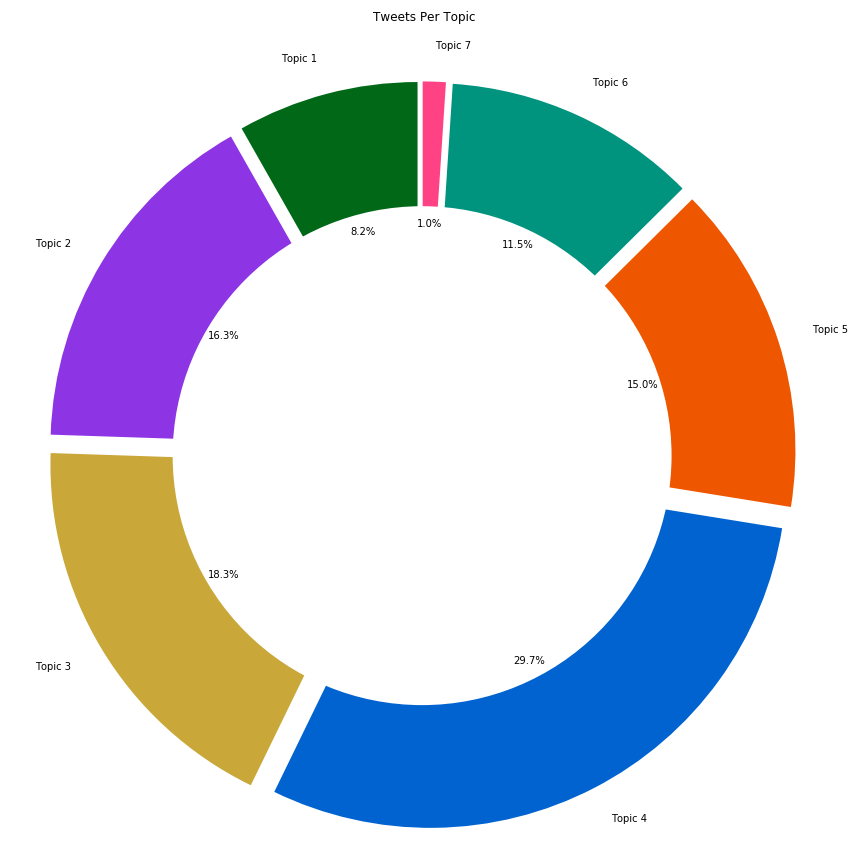
\includegraphics[scale=0.2]{Figures/topic_distribution}
    \caption[LDA Topic Distribution]{LDA Topic Distribution}
    \label{fig:topic_distribution}
    \end{figure}
\end{singlespacing}

\section{Topic Centrality}\label{sec:TopicCentrality}

\subsection{Total Network Topic Centrality}\label{sec:NetTopicCentrality}

	Define what it is, show the full graph again.

\subsection{Party Leader Topic Centrality}\label{sec:LeaderCentrality}

    Now, consider a fact stating that relation \texttt{r} is total, i.e.,

\subsection{Results}\label{sec:TopicCentralityResults}


\section{Stochastic Blockmodels}\label{sec:AdaptedSBMs}

As described in section \ref{sec:SBM}, stochastic blockmodels use edge densities
across and within blocks to generate random graph models
\cite{holland1983stochastic}. However, while users may belong to a certain
``party leader block'' or ``topic block''\footnote{In these cases, the blocks
would be users who would only engage with a certain party leader or topic, or
both.} to some degree, these cannot be known a priori and users can be members
of infinite combinations and mixtures of different blocks. As such, a novel
method for generating stochastic blockmodels was developed that approximated
edge densities and is specific to reproducing engagement graphs described in
section \ref{ch:GraphTheory}, where certain users produce objects (tweets,
songs, goods, etc...) and other users choose which ones to engage with. The
algorithm takes in 6 parameters: $n$, $tweet\_dist$, $k$, $m$,
$retweet\_histogram$, $\epsilon$ -- which are described in table
\ref{fig:SBMParameters}.

\begin{singlespacing}
    \begin{center}
    \begin{threeparttable}
    \caption{Adapted Stochastic Blockmodel Parameters}
    \label{fig:SBMParameters}
    \begin{small}
            \begin{tabular}{|l|l|l|}
            \hline
            \textbf{Parameter}              & \textbf{Type}                 & \textbf{Description} \\ \hline
            \emph{n}                        & $Integer$                     & \specialcell{The number of party leader vertices} \\ \hline
            \emph{tweet\_dist}              & $Tuple$                       & \specialcell{A tuple representing a normal distribution \\ $X \sim\mathcal{N}(\mu,\,\sigma^{2})$ that is sampled $n$ times to determine \\ the number of tweet vertices per party leader} \\ \hline
            \emph{$k$}                      & $Integer$                     & The number of topics that a tweet vertex can take on \\ \hline
            \emph{$m$}                      & $Integer$                     & The number of generic user vertices \\ \hline
            \emph{$retweet\_histogram$}     & $Histogram$\tnote{a}          & \specialcell{The distribution of retweets that is sampled $m$ \\ times to get the degree for each generic user} \\ \hline
            \emph{$\epsilon$}               & $Float \in \left[0-1\right]$  & \specialcell{The proportion of the time a generic user will choose \\ the greedy tweet-type\tnote{b}~ rather than choosing based \\ off of the edge probabilities}\\ \hline
            \end{tabular}
    \begin{tablenotes}
        \item[a]    As of March, 2020 -- this took the form as a Numpy histogram:
        a tuple containing the bin boundaries and corresponding densities.    
        \item[b]    For the models generated in this thesis a tweet-type could
        be its topic, who tweeted it, or its topic \emph{and} who tweeted it. 
    \end{tablenotes}
        \end{small}
    \end{threeparttable}
    \end{center}
\end{singlespacing}

 The algorithm generates the stochastic block model in three phases. First, all
 the party leader, tweet, and generic user vertices are generated based off of
 $n$, $tweet\_distribution$ and $m$, along with edges between the the party
 leader and tweet vertices. Second, topics are assigned to tweets randomly and
 $m$ samples of the $retweet\_histogram$ are generated to determine the retweet
 degree for each user, $D$. Finally, the algorithm loops through each generic
 user $i$ and retweets $D_{i}$ tweets. For each retweet a user makes, edge
 probabilities for each tweet-type are calculated based on the user's prior
 retweet history. The probability of forming an edge between user $i$ and a
 tweet-type $t$, given edge probabilities $e_{i}$, is given by the
 policy\footnote{Policy in this context refers to the probability of choosing an
 action from some set of possible actions and is denoted by $\pi$; all other
 mentions to policy in this thesis refer to categories of messages.} $\pi$ in
 equation \ref{equation:policy_equation}. This is a variation of the
 $\epsilon$-$greedy$ algorithm, where the tweet-type with the highest
 probability is chosen $\epsilon$ percent of the time, and $(1-\epsilon)$
 percent of the time tweets are chosen based off of $e_{i}$. After each edge is
 formed user $i$'s retweet history is updated.
 
\begin{numcases}{\text{$\pi(t|e_{i})$}}\label{equation:policy_equation}
    \epsilon                & if $t = argmax_{t} e_{i}$ \notag \\
    (1-\epsilon)e_{it}    & otherwise \notag
\end{numcases}

While initially the edge probabilities for a user $i$ would be proportional to
their retweet history\footnote{This can be done efficiently by taking the
$softmax$ of the retweet history.}, section \ref{sec:DeepSBMs} demonstrates
how more nuanced edge probabilities can be developed with deep stochastic
blockmodels. This is formalized in algorithm \ref{algorithm:SBM}.

\begin{singlespacing}
\begin{algorithm}[H]
    \SetAlgoLined
    \KwResult{A stochastically generated political engagment graph}
    initialize $G$ as an empty graph\;
    initialize $T$ as an array of all different tweet-types\;
    initialize $n$ party leader vertices in $G$\;
    initialize $m$ generic user vertices in $G$\;
    \For{$i\leftarrow 1$ \KwTo $n$}{
        initialize $X \sim\mathcal{N}(\mu,\,\sigma^{2})$ tweet vertices in $G$\;
        assign tweet vertices random topics from $[1,...,k]$\;
        add edges from tweet vertices to party leader $i$\;
    }
    generate retweet degree array $D$ of size $m$ by sampling $retweet\_histogram$\;
    \For{$i\leftarrow 1$ \KwTo $m$}{
        initialize $user\_history$ array of size $|T|$ with all 0s\;
        \For{$j\leftarrow 1$ \KwTo $D_{i}$}{
            generate edge probabilities $e_{i}$\;
            add an edge from user $i$ to a tweet of tweet-type $t$ based on $\pi(t|e_{i})$\;
            $user\_history_{t}+=1$
        } 
     }
     \KwRet{$G$}
     \caption{Stochastic blockmodel for modelling political engagement}
     \label{algorithm:SBM}
\end{algorithm}
\end{singlespacing}


\subsubsection{Deep Stochastic Blockmodels for Modelling Political Engagement}\label{sec:DeepSBMs}

As discussed in section \ref{sec:AdaptedSBMs}, the edge probabilities for a user
retweeting a tweet-type can be calculated in various ways. A further nuance that
can be added is incorporating real world data into the edge probability
calculation. Data used to generate the complete political engagement graph in
figure \ref{fig:og_graph} was used to train two feed-forward artificial neural
networks (ANN) to aid in the edge probability calculation: one that predicts the next
party leader a user would tweet given the prior party leaders they had
retweeted, and one that predicts which topic a user would retweet given the
previous topics of tweets that user had retweeted. Figure \ref{fig:confusion_matrices} shows the
confusion matrices for these two ANNs. Both ANNs attained between 85-87\% accuracy.

\begin{singlespacing}
    \begin{figure}
        \centering
        \begin{tabular}{cc}
          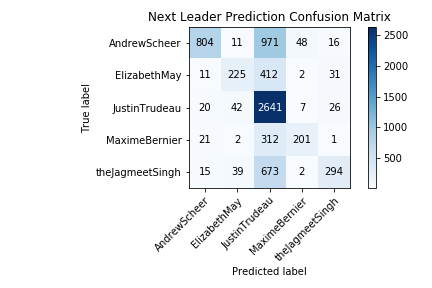
\includegraphics[width=60mm]{Figures/next_leader_CM}
          &
          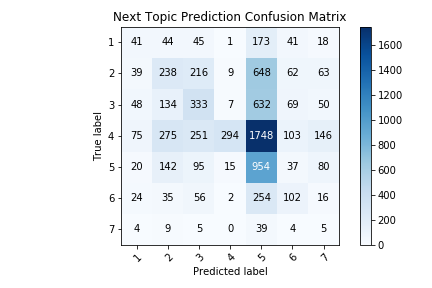
\includegraphics[width=60mm]{Figures/next_topic_CM}
          \\
        (a) ``Next Leader'' Confusion Matrix & (b) ``Next Topic'' Confusion Matrix \\[6pt]
        \end{tabular}
        \caption[ANN Confusion Matrices]{ANN Confusion Matrices}
        \label{fig:confusion_matrices}
    \end{figure}
\end{singlespacing}

Sections \ref{sec:SPLBM}, \ref{sec:STBM} and \ref{sec:SHBM} will demonstrate
both the utility of these ANNs in generating the stochastic blockmodels in
comparison to the standard edge probability calculation.

\subsection{Stochastic Party Leader Blockmodel}\label{sec:SPLBM}

The stochastic party leader model generates user behaviour only taking into
account the previous party leaders each user had engaged with prior. The
tweet-types therefore are all the different party leaders that could be
retweeted and $e_{i}$ represents the weights of retweeting each party leader.
For each user, when deciding which tweet they are to retweet, their retweet
history is converted into a probability distribution (ex.\
$user\_history_{i}=[JT=0,AS=1,JS=3,EM=2,MB=0]$ generates
$e_{i}=[JT=0.09,AS=0.19,JS=0.36,EM=0.27,MB=0.09]$). In this sense, it models a
world in which politically engaged Twitter users only engage along the axis of
party leaders, with a complete disregard for the topics tweeted about. Figure
\ref{fig:stochastic_party_leader_model} shows two examples of stochastic party
leader blockmodels: one in which edge probabilities are proportional to the
number of times that user's retweeted each party leader, and one in which edge
probabilities are determined with the ANN described in section
\ref{sec:DeepSBMs}.

\begin{singlespacing}
    \begin{figure}
        \centering
        \begin{tabular}{cc}
          \includegraphics[width=50mm]{Figures/simple_stochastic_party_leader_model}
          &
          \includegraphics[width=50mm]{Figures/ann_stochastic_party_leader_model}
          \\
        (a) Simple Stochastic Party Leader Blockmodel & (b) ANN Adaption\\[6pt]
        \end{tabular}
        \caption[Stochastic Party Leader Blockmodels]{Stochastic Party Leader Blockmodels}
        \label{fig:stochastic_party_leader_model}
    \end{figure}
\end{singlespacing}

\subsection{Stochastic Topic Blockmodel}\label{sec:STBM}

Conversely, the stochastic topic blockmodel models a world in which politically
engaged Twitter users only engage along the axis of topics. In this case, the
tweet-types are the various different topics that a user can engage with. Here,
the tweet-type history of a user is converted into a probability distribution,
and with a probability of $\epsilon$, that user will retweet the topic with the
highest activation -- regardless of which party leader tweeted it. Figure
\ref{fig:stochastic_topic_model} shows two examples of stochastic topic
blockmodels: in which edge probabilities are proportional to a user's topic
retweet history, and one in which edge probabilities are determined with the ANN
described in section \ref{sec:DeepSBMs}.

\begin{singlespacing}
    \begin{figure}
        \centering
        \begin{tabular}{cc}
          \includegraphics[width=50mm]{Figures/simple_stochastic_topic_model} &
          \includegraphics[width=50mm]{Figures/ann_stochastic_topic_model} \\
        (a) Simple Stochastic Topic Blockmodel & (b) ANN Adaption\\[6pt]
        \end{tabular}
        \caption[Stochastic Topic Blockmodels]{Stochastic Topic Blockmodels}
        \label{fig:stochastic_topic_model}
    \end{figure}
\end{singlespacing}

\subsection{Stochastic Hybrid Blockmodel}\label{sec:SHBM}

The final model developed is a hybrid of the stochastic party leader block
model, and the stochastic topic blockmodel. Here, two history vectors for each
user are captured -- the $n$ dimensional party leader history vector, and the
$k$ dimensional topic history vector. After each respective vector is converted
into a probability distribution, the edge probability of topic $i$ by party
leader $j$ is determined by some constant $\alpha$\footnote{This has no relation
to the parameter $\alpha$ referred to in section \ref{sec:LDA}} and the
function:

\begin{equation}
    edge\_probability(party leader=i, topic=j)=\alpha P(i)+(1-\alpha)P(j)
\end{equation}

Where $P(i)$ is index $i$ of that user's \emph{party leader} probability
distribution, $P(j)$ is index $j$ of that user's \emph{topic} probability
distribution, and $\alpha$ is some constant that determines the relative
weighting of the two. As $\alpha$ approaches $1$, the hybrid model becomes
equivalent to the stochastic party leader blockmodel -- and as $\alpha$
approaches $0$ the model approaches the stochastic topic blockmodel. This model
then generates different ``worlds'' in which users' political engagement falls
on the spectrum from only caring about \emph{party leaders} to only caring about
\emph{topics}.

\begin{singlespacing}
    \begin{figure}
        \centering
        \begin{tabular}{cc}
          \includegraphics[width=50mm]{Figures/standard_SHBm_ex} &
          \includegraphics[width=50mm]{Figures/deep_SHBm_ex} \\
        (a) Standard SHBm ($\alpha$=0.60) & (b) Deep SHBm ($\alpha$=0.60)\\[6pt]
        \end{tabular}
        \caption[Stochastic Topic Blockmodels]{Stochastic Topic Blockmodels}
        \label{fig:SHBm_examples}
    \end{figure}
\end{singlespacing}

\subsection{NetLSD for Describing Political Engagement}\label{sec:NetLSDForSBM}

The final objective of comparing the relative importance of topics and party
leaders in driving political engagement requires comparing the structure of
target graph shown in \ref{ch:GraphTheory}, and various hybrid models generated
with different values of $\alpha$. Using the Network Laplacian Spectral
Descriptor described in section \ref{sec:NetLSD} by Tsitsulin et al. the optimal
alpha value can be determined in a scale-adaptive, size-invariant, and
permutation-invariant manner \cite{netlsd}.

Given the $O(n^{3})$ complexity involved in calculating the eigenvalues of a
graphs normalized Laplacian matrix it is advantageous to generate sufficiently
small hybrid models when fitting them to the original engagement graph (see
figure \ref{fig:og_graph}). To determine how large a graph of this nature needs
to be to capture its underlying structure -- tweets of the original graph were
sampled, keeping all the retweet edges, and then compared to the heat trace
signature of the original graph. This is shown graphically in figure
\ref{fig:dist_from_original_graph_over_sample_size}, the x-axis represents how
many tweets \emph{per party leader} were sampled from the original graph and the
y-axis represents the $L_{2}$ distance from the original engagement graph's heat
trace signature. 

\begin{singlespacing}
    \begin{figure}[H]
    \centering
    \begin{tabular}{cc}
        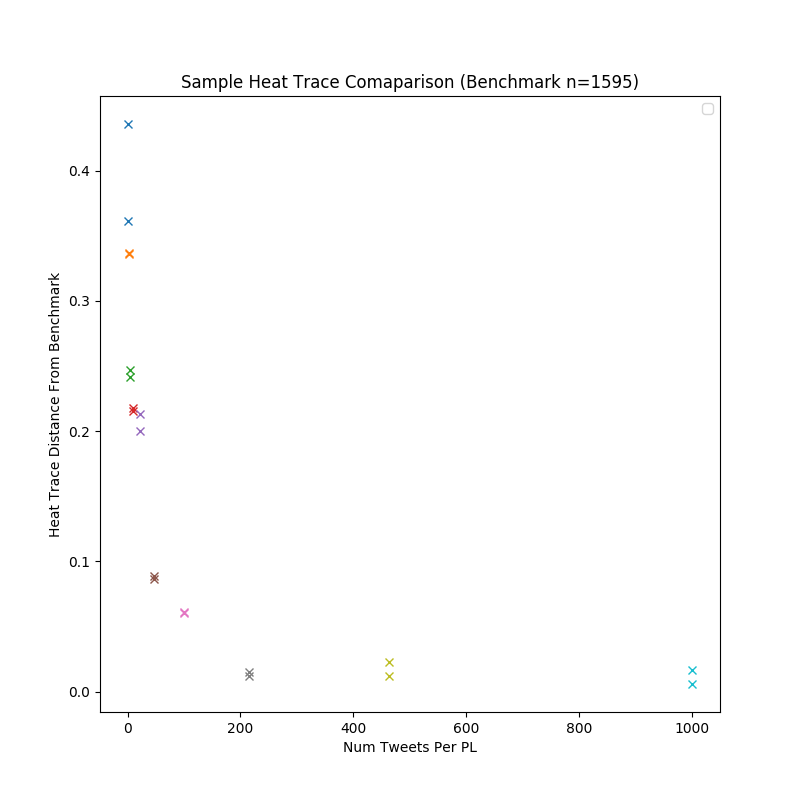
\includegraphics[width=50mm]{Figures/dist_from_original_graph_over_sample_size} &
        \includegraphics[width=50mm]{Figures/sampled_graph} \\
        (a) Heat Trace Signature Distances & (b) Engagement Graph (215 Tweets per PL)\\[6pt]
    \end{tabular}
    \caption[Heat Trace Signature Distance as a Function of Graph Sample Size]{Heat Trace Signature Distance as a Function of Graph Sample Size}
    \label{fig:dist_from_original_graph_over_sample_size}
    \end{figure}
\end{singlespacing}

As can be seen from figure \ref{fig:dist_from_original_graph_over_sample_size},
there are diminishing returns for graphs with more than 215 tweets per party
leader. Therefore, for each of the party leader vertices generated with the
hybrid models -- each one generated a number of tweets by a random variable $X$
that is distributed normally where $X \sim
\mathcal{N}(\mu=215,\,\sigma^{2}=70)$.

\subsection{Results}\label{sec:SBMsResults}

The stochastic hybrid blockmodel (SHBm) gives the ability to define different
``worlds'' in which policy and party leaders drive engagement to different
degrees. NetLSD gives the ability to compare the structural similarity of graphs
in a scale-adaptive, size-invariant, and permutation-invariant manner. By
performing a sweep of different $\alpha$ values for the hybrid models, and
measuring which one produces the heat trace signature with the smallest $L_2$
distance to the original graph, the final objective of putting Ezra Klein's
hypothesis to task can be achieved. All graphs were generated with $n=5$, 
$k=7$, $tweet\_dist=(\mu=215,\,\sigma^{2}=70)$, $m=8826$, $retweet\_histogram$
derived from the original engagement graph, and $\epsilon=0.95$. $\alpha$ values
ranging between 0 and 1, with increments of 0.05 were used to generate the
different hybrid models. Four models were generated per $\alpha$ and the mean
distance was used to determine the final distance.

The results of this experiment are striking: in both the deep SHBm, which uses
the ANN to calculate edge probabilities, and the standard SHBm, which makes
edge probabilities proportional to the user's retweet history, it is clear that
both \emph{what} the message is and \emph{who} tweeted the message drive
political engagement. The standard SHBm shows a clear trend where $\alpha$
values that privilege policy over party leader, or vice versa, have a further
distance from original engagement graph than ones that blend the two. These hybrid models
had the best fit when $\alpha=0.6$. The deep SHBm had an optimal fit when
$\alpha=0.4$. The full tabular data is shown in table
\ref{fig:tab_SHBm_results}, and the results are visualized in figure \ref{fig:SHBm_results}.

\begin{singlespacing}
    \begin{figure}
        \centering
        \begin{tabular}{cc}
            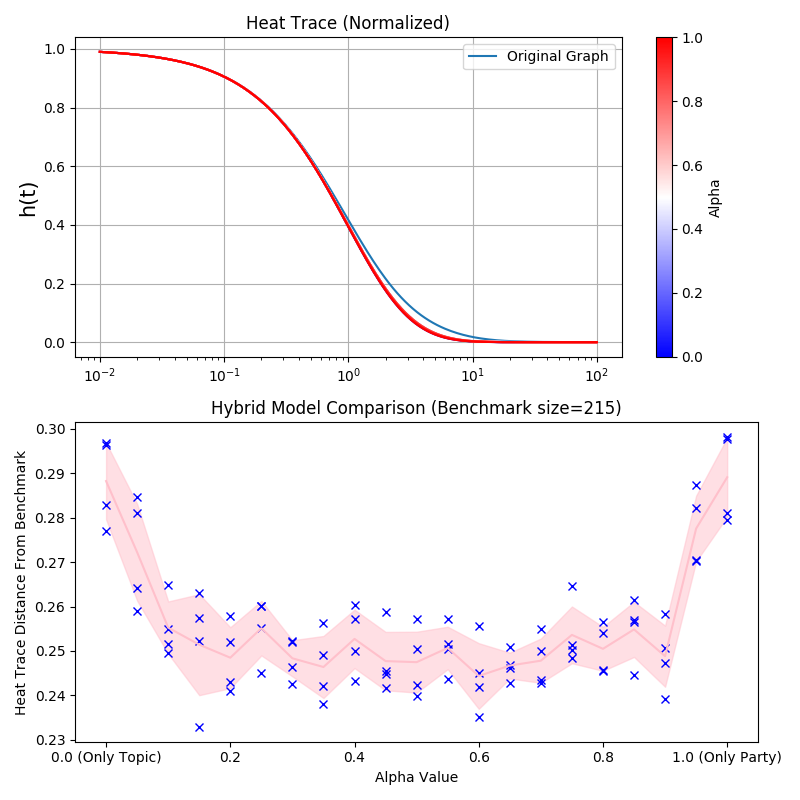
\includegraphics[scale=0.3]{Figures/standard_heat_trace_plot} &
            \includegraphics[scale=0.3]{Figures/ann_heat_trace_plot} \\
            (a) Standard SHBm $L_{2}$ Plots & (b) Deep SHBm $L_{2}$ Plots\\[6pt]
        \end{tabular}
        \caption[Stochastic Topic Blockmodels]{Stochastic Topic Blockmodels}
        \label{fig:SHBm_results}
    \end{figure}
\end{singlespacing}

\begin{singlespacing}
    \begin{center}
    \begin{threeparttable}
    \caption{Results of NetLSD Comparison of SHBm Models}
    \label{fig:tab_SHBm_results}\begin{small}
        \begin{tabular}{|l|c|c|c|c|c|c|c|} \hline

        \multicolumn{1}{|c|}{} & \multicolumn{3}{|c|}{Standard SHBm} & \multicolumn{3}{|c|}{Deep SHBm} \\ \hline

        \multicolumn{1}{|c|}{$\alpha$} & Min $L_{2}$ & Mean $L_{2}$ & $\sigma^{2}$  & Min $L_{2}$ &  Mean $L_{2}$ & $\sigma^{2}$ \\  \cline{6-7}

        \hline
            0.00  & 0.2648 & 0.2756 & 0.0083   &  0.2173 & 0.2276 & 0.0062 \\
        \hline
            0.05  & 0.2475 & 0.2603 & 0.0104   &  0.2111 & 0.2201 & 0.0073 \\
        \hline
            0.10  & 0.2385 & 0.2440 & 0.0057   &  0.2030 & 0.2231 & 0.0117 \\
        \hline
            0.15  & \textbf{0.2225} & 0.2403 & 0.0109   &  0.2176 & 0.2217 & 0.0061 \\
        \hline
            0.20  & 0.2303 & 0.2375 & 0.0066   &  0.2210 & 0.2260 & 0.0037 \\
        \hline
            0.25  & 0.2343 & 0.2439 & 0.0059   &  0.2172 & 0.2241 & 0.0067 \\
        \hline
            0.30  & 0.2319 & 0.2374 & 0.0039   &  0.2207 & 0.2260 & 0.0058 \\
        \hline
            0.35  & 0.2274 & 0.2355 & 0.0067   &  \textbf{0.2022} & 0.2174 & 0.0095 \\
        \hline
            0.40  & 0.2328 & 0.2418 & 0.0063   &  0.2096 & \textbf{0.2134} & 0.0031 \\
        \hline
            0.45  & 0.2313 & 0.2370 & 0.0063   &  0.2181 & 0.2257 & 0.0067 \\
        \hline
            0.50  & 0.2296 & 0.2368 & 0.0066   &  0.2255 & 0.2355 & 0.0085 \\
        \hline
            0.55  & 0.2329 & 0.2396 & 0.0046   &  0.2440 & 0.2565 & 0.0116 \\
        \hline
            0.60  & 0.2246 & \textbf{0.2336} & 0.0071   &  0.2249 & 0.2508 & 0.0187 \\
        \hline
            0.65  & 0.2320 & 0.2358 & 0.0028   &  0.2260 & 0.2418 & 0.0125 \\
        \hline
            0.70  & 0.2320 & 0.2369 & 0.0048   &  0.2260 & 0.2418 & 0.0125 \\
        \hline
            0.75  & 0.2374 & 0.2425 & 0.0061   &  0.2610 & 0.2718 & 0.0079 \\
        \hline
            0.80  & 0.2347 & 0.2394 & 0.0047   &  0.2603 & 0.2692 & 0.0062 \\
        \hline
            0.85  & 0.2338 & 0.2436 & 0.0060   &  0.2484 & 0.2597 & 0.0081 \\
        \hline
            0.90  & 0.2286 & 0.2378 & 0.0066   &  0.2604 & 0.2684 & 0.0058 \\
        \hline
            0.95  & 0.2584 & 0.2654 & 0.0071   &  0.2432 & 0.2581 & 0.0111 \\
        \hline
            1.00  & 0.2672 & 0.2765 & 0.0085   &  0.2506 & 0.2611 & 0.0098 \\
        \hline
        \end{tabular}
    \end{small}
    \end{threeparttable}
    \end{center}
    \end{singlespacing}




\chapter{Summary and Conclusions}\label{ch:Conclusion}

\section{Summary}

\section{Other Work}

\subsection{International Network for Social Network Analysis}

\section{Future Work}

\section{Conclusion}


%*************************************************************************************************************
% BIBLIOGRAPHY
%*************************************************************************************************************
\bibliographystyle{plain}
\bibliography{thesis}
\end{document}
